\documentclass{article}

% Symbols
\usepackage{amsfonts, amsthm}
\usepackage{upgreek}
\usepackage{physics}
\usepackage{cancel}
\usepackage{amssymb, latexsym, amsmath}
\usepackage{import}
\usepackage[table,xcdraw]{xcolor}

%Algorithms
\usepackage[ruled,lined,linesnumbered,commentsnumbered]{algorithm2e}

%% Identación
\setlength{\parindent}{0cm}

% Código
\newcommand{\code}[1]{\textcolor{white!25!black}{\texttt{#1}}}
\usepackage{listings}

%AMS
\usepackage{amsthm}
\newtheorem{algo-thm}{Algoritmo}

% Graphics
\usepackage{graphicx}
\usepackage{pgf}

% Margins
\addtolength{\voffset}{-1.5cm}
\addtolength{\hoffset}{-1.5cm}
\addtolength{\textwidth}{3cm}
\addtolength{\textheight}{3cm}

%Header-Footer
\usepackage{fancyhdr}
\renewcommand{\headrulewidth}{1pt}

\newcommand{\set}[1]{
  \left\{ #1 \right\}
}

\footskip = 50pt
\renewcommand{\headrulewidth}{1pt}

\pagestyle{fancyplain}

\begin{document}
\title{UNIVERSIDAD NACIONAL AUT\'ONOMA DE M\'EXICO\\ Facultad de Ciencias}
\author{Equipo NullPointerException:\\
        Adri\'an Aguilera Moreno   - 421005200\\
        Diego Angel Rosas Franco   - 318165330 \\
        Marco Antonio Rivera Silva - 318183583}
\date{}
\maketitle
\begin{center}
  
\includegraphics[scale=0.20]{./Portada/Portada}\\[0.4cm]
  \Large
  \bf{Modelado y programación}
  \normalsize
\end{center}
\newpage
\fancyhead[r]{ Modelado y programación 2022-2}


\section*{\LARGE{Proyecto 02}}

\subsection*{Contexto}
La Facultad de Ciencias algunas veces se asocia con ser un lugar gris y deprimente donde sus estudiantes, por esta misma razón, se ven desmotivados muchas veces.
Para ayudar a los estudiantes y crear una perspectiva distinta de la facultad, decidimos crear un juego ambientado en ella.. 
En este juego podremos recorrer determinadas zonas de la facultad, enfrentar a personajes icónicos y ver otro lado distinto de la facultad.
Por cuestiones de tiempo, solo se establecerá la lógica del combate y de la exploración del mapa. Se planea dejar las bases listas para realizar un juego entretenido con una posible historia que permita explorar y descubrir historias de la facultad de una manera única.
Aspectos generales del juego:











\begin{itemize}
\item Se tratará de un juego RPG por turnos.
\item Inicialmente podrás nombrar a tu jugador y elegir la carrera a la que pertenece.
  \begin{itemize}
  \item Según la carrera elegida se le otorgará una
    habilidad única a usar durante su estancia en la Facultad.
  \item Las carreras a elegir son:
    \begin{itemize}
    \item Ciencias de la Computación.
    \item Matemáticas.
    \item Actuaría.
    \item Biología.
    \item Física.
    \end{itemize}
  \end{itemize}
\item El jugador tendrá, sin importar su carrera, dos ataques por defecto: Ataque Débil y Ataque Fuerte.
\item Sobre los ataques:
  \begin{itemize}
  \item El usuario contará con 4 ranuras de ataques, dos con los ataques por defecto, una con su habilidad
    especial única (por carrera) y una cuarta donde se planea que a futuro esta pueda ser intercambiada por
    ataques que vaya consiguiendo el jugador durante la partida.
  \end{itemize}
\item El jugador podrá recorrer algunos lugares de la facultad.
  \begin{itemize}
  \item Inicialmente el jugador empezará en una entrada de la facultad.
  \item Encontrará jefes en lugares específicos de la Facultad.
  \end{itemize}
\item Los jefes serán personajes icónicos de la facultad.
\item El jugador podrá elegir a qué jefes enfrentar, es decir, será un mundo abierto
  (dentro de las limitaciones topográficas de la facultad).
\item El combate será por turnos donde cada jefe tendrá una habilidad única que a
  futuro el jugador podrá “aprenderla”.
\item Inicialmente se contará con un jefe al cual enfrentar y dos zonas que podrá explorar:
  la planta baja del edificio Tlahuizcalpan y la entrada del busto de Darwin.
\end{itemize}

\newpage
\subsection*{Justificación de uso de patrones:}
\subsubsection*{Strategy}
Este \textit{patrón de diseño} se implementa en los \code{AtaqueUnico}'s, donde la clase Jugador tendrá un "Ataque Especial" que podrá ir cambiando durante el juego. Este Ataque Especial podrá cambiar entre distintos tipos de ataque:
\begin{itemize}
\item \code{AtaqueBloqueoTurno}: Ataque que permite omitir un turno del oponente para realizar dos ataques seguidos (donde el primero es el de tipo bloqueo turno).

\item \code{AtaqueDanioExagerado}: Se trata de un ataque con un daño mucho mayor que los otros ataques.

\item \code{AtaqueDrenarVida}: Ataque que drenará vida del oponente en los siguientes n turnos.

\item \code{AtaquePotenciado}: Este ataque potenciará n turnos todos los ataques del jugador. Con potenciar se refiere a que aumentará el daño.

\end{itemize}

Decidimos usar Strategy porque el Ataque Especial esta pensado para cambiar en tiempo de ejecución y que el jugador pudiera usar un solo Ataque Especial a la vez de los que fuera adquiriendo a lo largo del juego.

\subsubsection*{State}
Este \textit{patrón de diseño} se implementa dos veces en el proyecto, estas son:
\begin{itemize}
\item[$*$)] \textbf{Estados del Jugador:}
  Se decidió usar State porque este nos permitiría manejar a futuro el comportamiento del jugador en el mapa, tanto para recorrerlo, como interactuar con elementos del mapa (aparte de los jefes). Además de que nos permitiría tener una restricción y por lo tanto una validación en lo que se podía hacer con el jugador en el mapa.

\item[$*$)] \textbf{Estados de la interfaz:}
  Su función es dibujar los diferentes mapas desde los estados de título, pelea,
  jugar, inventario y pausa. Así, los diferentes estados tienen diferentes funciones,
  estas son:
  \begin{itemize}
  \item \code{EstadoPelea}: Se usa para entrar en pelea con algún jefe.
  \item \code{EstadoJugar}: Se usa para entrar en el estado principal de juego.
  \item \code{EstadoPausa}: Se utiliza para pausar los movimientos en el mapa.
  \item \code{EstadoTitulo}: Se utiliza para entrar en Estado Titulo y dibujar el 
  \item \code{EleccionCarrera}: Se utiliza para entrar en Estado Titulo y dibujar el titulo.
  \item \code{EstadorInventario}: Se usa para entrar en el Estado Inventario y mostrar el inventario. 
  \end{itemize}
\end{itemize}
\subsubsection*{Facade}
Este \textit{patrón de diseño} se utiliza en la clase \code{Main} que es la fachada
de las clases:
\begin{itemize}
\item \code{JFrame}.
\item \code{PanelJuego}.
\end{itemize}
\subsubsection*{Iterator}
Este \textit{patrón de diseño} se utiliza en la clase \code{Jugador} para
recorrer el \code{HashMap} utilizado para guardar los ataques adquiridos
por el jugador, y en la clase \code{TiendaAtaquesEspeciales} para recorrer
la lista \code{LinkedList} que guarda los ataques de la tienda. Se decidió utilizar Iterator porque se consideró que a futuro el juego tuviese distintas tiendas especializadas, por ejemplo, una para Items, otra para Ataques de ciertos tipos, etc. Donde cada tienda tendría su propia forma de almacenar sus datos, pero para no exponer dichas formas recurrimos a Iterator.

\subsection*{Otros patrones que se pudieron usar:}
\subsubsection*{Singleton}
Nos percatamos en que podiamos usar el patrón \code{Singleton} con las clases
\code{AtaqueDebil} y \code{AtaqueFuerte}, pues debe comportarse de la misma
manera para todos los jugadores. Sin embargo, una modificación a este tipo
de \code{Ataque} modificaría el ataque para los demás jugadores en el sistema,
pues se crearía siempre una instancia única y las demás sería copias propias.

\subsubsection*{Proxy}
En la parte de devolver los ataques de los jefe y jugadores pudimos utilizar el
patrón \code{Proxy}, pues podemos dar una instancia \code{Proxy} y no directamente
la instancia al objeto y así poder evitar accesos y modificaciones indeseadas.
Sin embargo, esto lo pudimos resolver de manera más fácil al emplear el patrón
\code{Iterator}.

\subsubsection*{Decorator}
Pensamos en usar Decorator para crear los tipos de ataques, pero esto complicaría la forma en que los estabamos pensando pues un ataque podía ser de un solo tipo, y no sería tan facil ver quien era el ataque original.


\newpage
\subsection*{Instrucciones de instalación, compilación y ejecución.}
Se dará por hecho que el usuario sabe moverse en terminal.

\subsubsection*{Requerimientos previos:}
\begin{itemize}
\item[-] Se debe contar con una versión de Java $17.0.1$ o superior en
  su computadora. De preferencia la versión más reciente.
\end{itemize}

\subsubsection*{Ejecución del proyecto:}
\begin{itemize}
\item[-] Si está leyendo esto significa que desempaquetó con éxito el proyecto.
\item[-] Abra su terminal y diríjase a la ruta donde desempaquetó el proyecto.
\item[-] Una vez estando en la ruta
  
  \code{CienciasException\_NullPointerException},
  
  diríjase a

  \code{CienciasException\_NullPointerException/src/fciencias/modelado/}
\item[-] Ejecute: “\code{javac Main.java}”, esto generará los .class del proyecto. Esto puede
  tardar unos segundos, por lo que se pide tener paciencia.
\item[-] Ejecute: “\code{java Main}”, esto ejecutará el proyecto mostrándole el menú del mismo.
\end{itemize}

\subsubsection*{Ingreso al sistema:}
La interfaz mostrará la pantalla principal con el titulo del juego, y las opciones de "Nuevo juego", "Proximamente" y "Salir".
Se podra mover en las opciones con las teclas 'w' y 's'. Y para elejir una deberá presionar la tecla "Enter".
En cuanto se muestre este menú, podrá encontrar una ventana emergente donde deberá ingresar su nombre despues de dar clic al botón "Haz clic en mi para poner tu nombre". Este nombre será el nombre de tu personaje.
Cuando se elija la opción "Nuevo juego" podrá seleccionar la carrera de su personaje, dependiendo de la carrera elejida el personaje obtendrá un ataque Unico de su carrera, por ejemplo: Apartismo (Actuaria), Calculismo (Matemáticas), entre otros.
Una vez elejida la carrera inicia el juego y podrá moverse libremente en el mapa de la facultad con las teclas awsd, donde: 'a'=izquierda, 'w'=arriba, 's'=abajo y 'd'=derecha.
Cuando se entre en una batalla podra seleccionar el ataque a realizar y para continuar deberá presionar la tecla de "SPACE".
Para la ventana de la tienda que también muestra los ataques especiales adquiridos se podrá salir presionando "ESC".
En el mapa puedes poner Pausa presionando la tecla 'p'.
Por el momento se cuenta con una experiencia inmersiva tipo SAO (Sword Art Online), una vez empieza no hay forma de salir.

\newpage
\subsection*{Diagrama UML:}
\begin{center}
  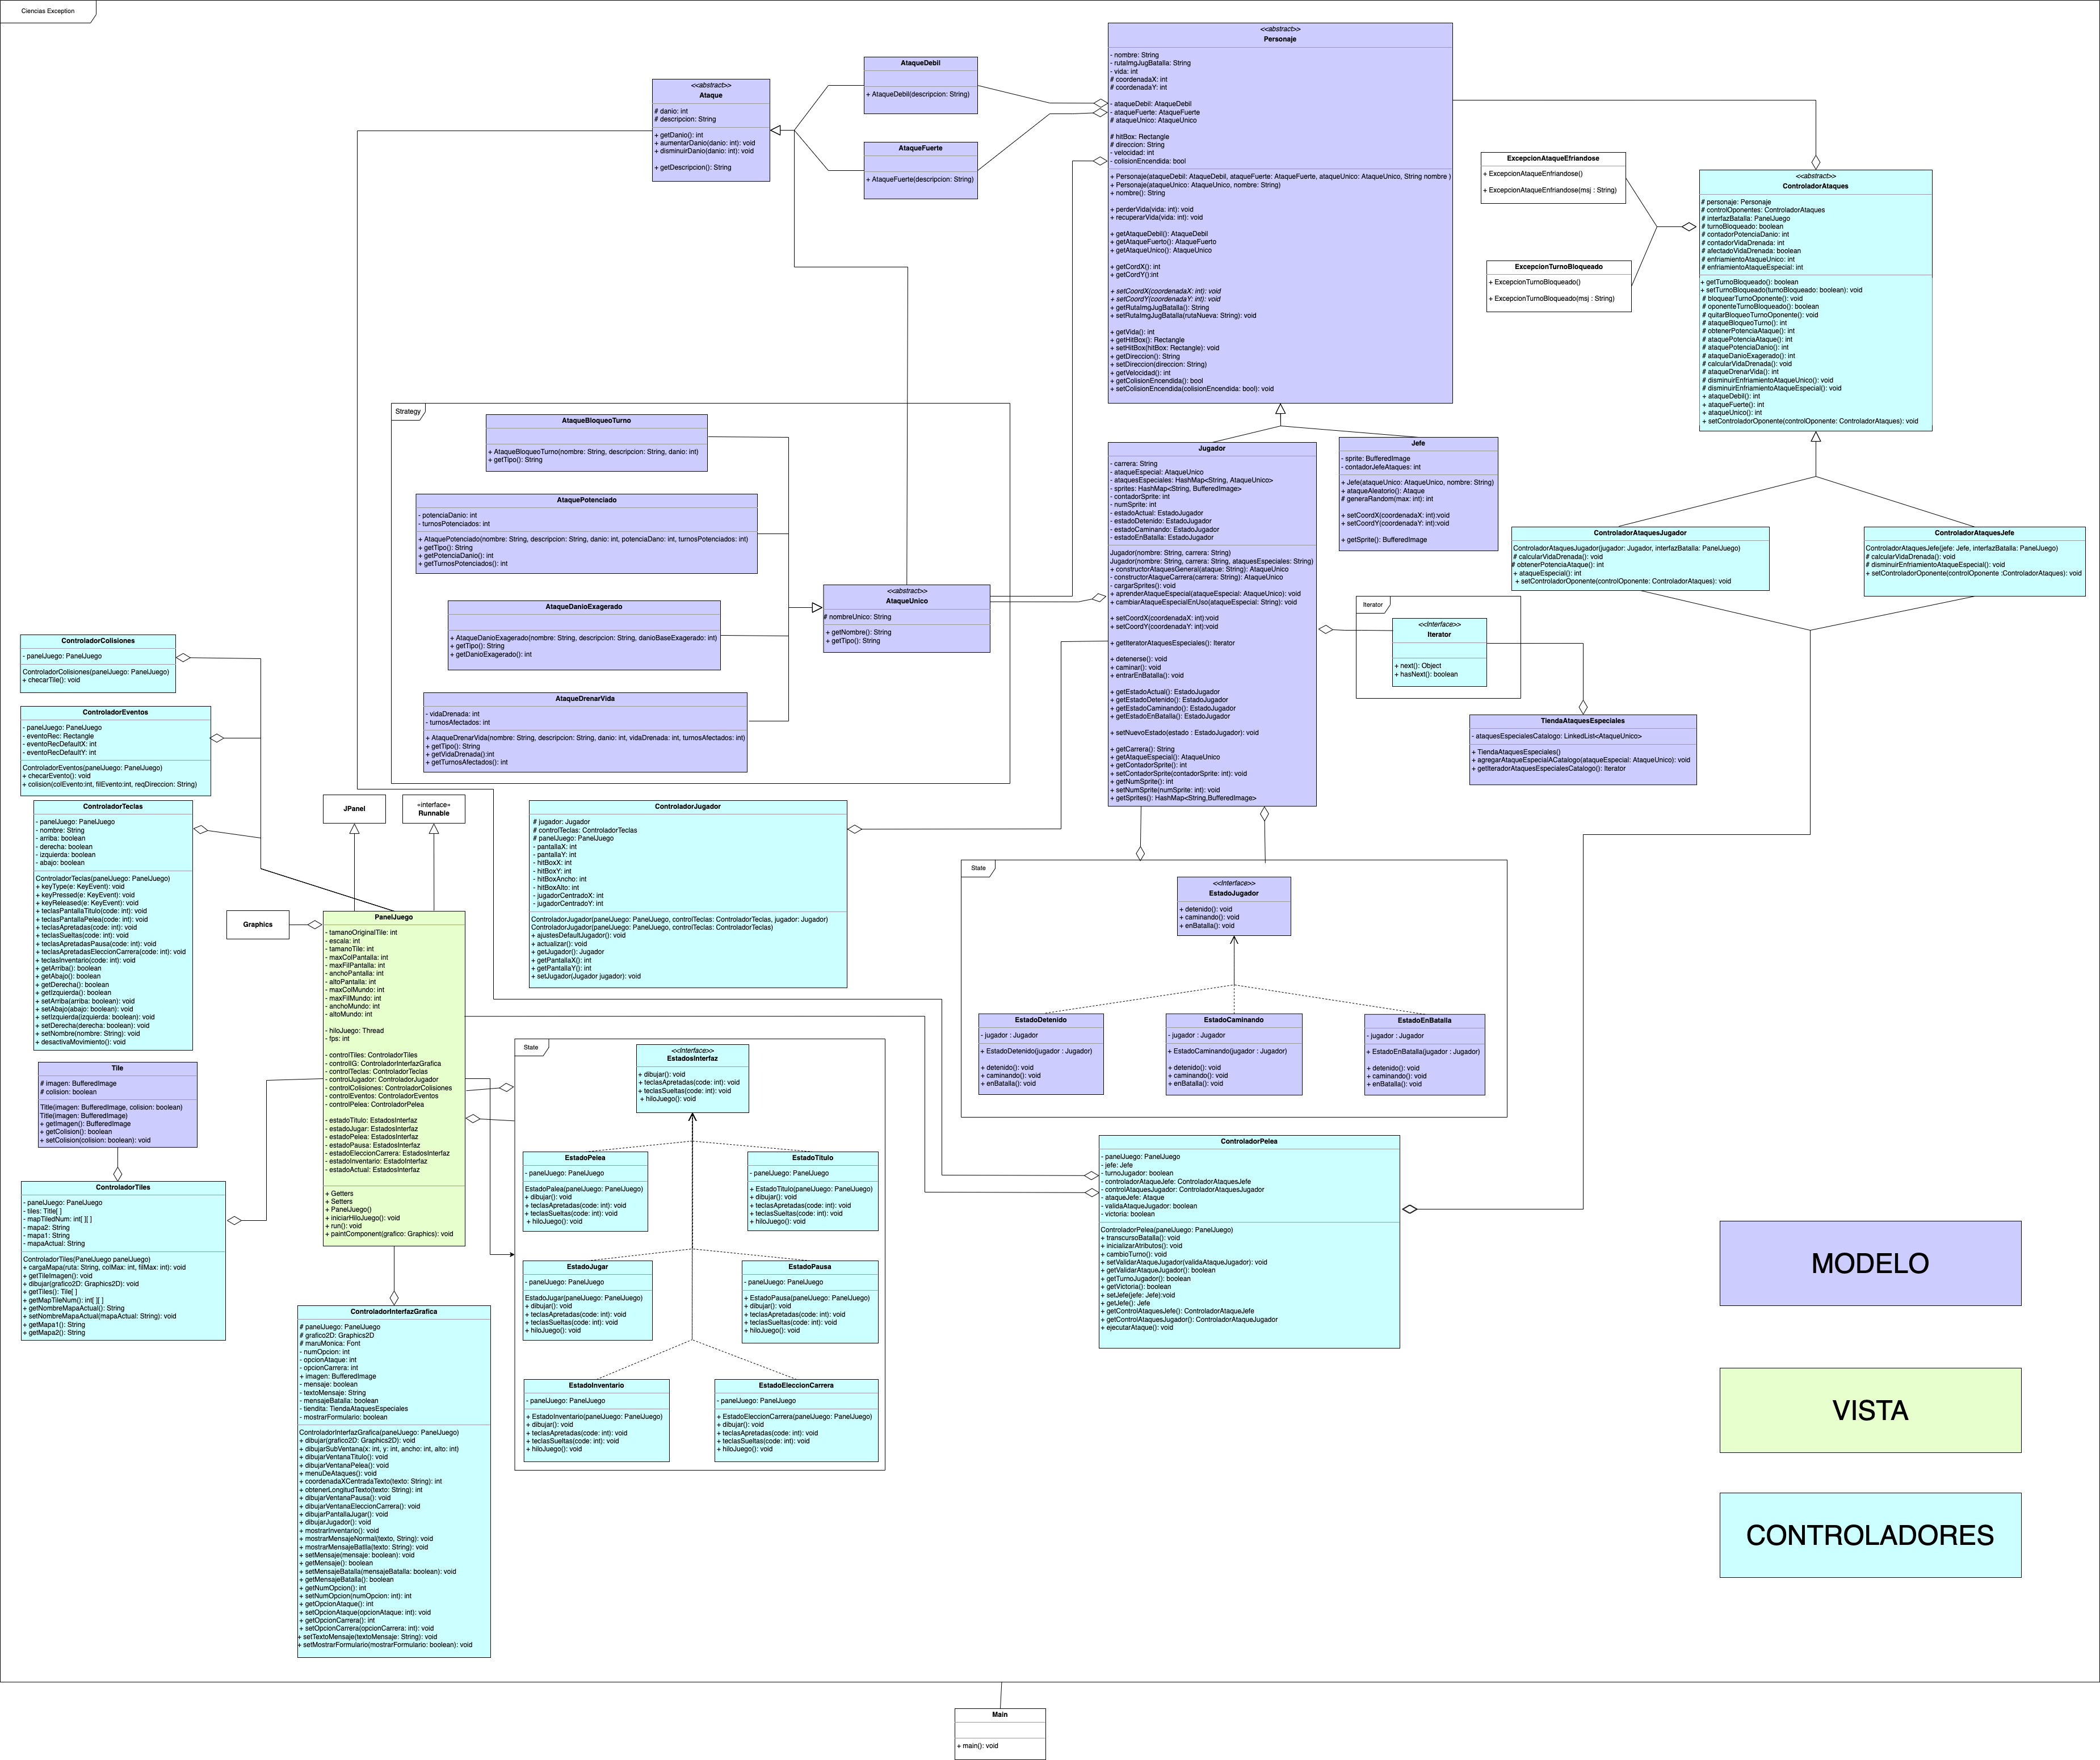
\includegraphics[scale=0.10]{./CienciasExceptionUML.png}
\end{center}

\subsection*{Diagrama de Casos de Uso:}
\begin{center}
  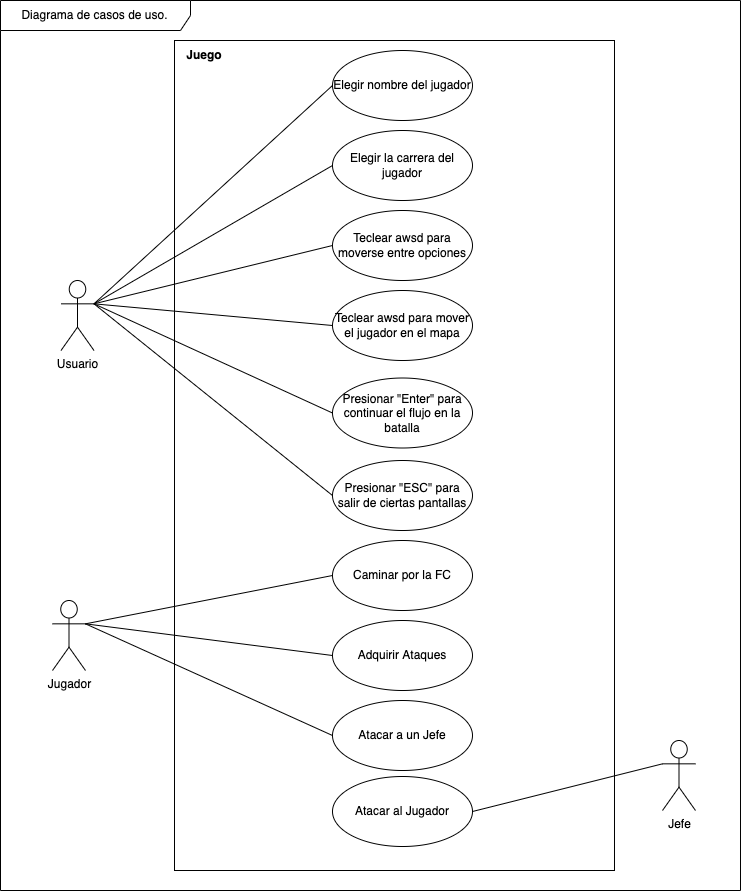
\includegraphics[scale=0.18]{./DiagramaDeCasosDeUso.png}
\end{center}

\subsection*{Diagrama de Estados:}
\begin{center}
  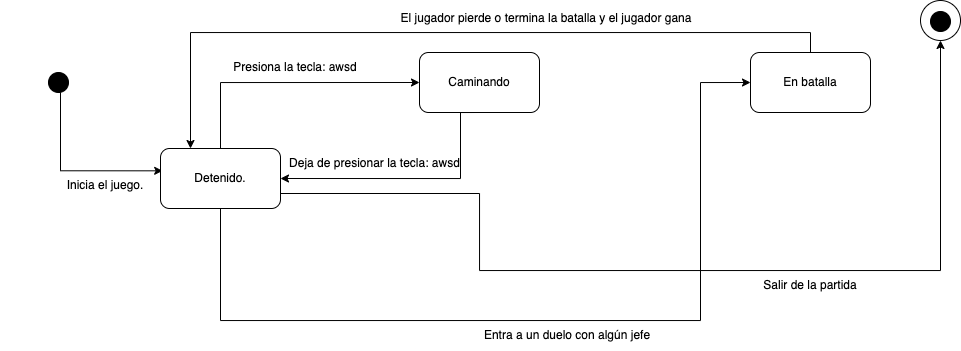
\includegraphics[scale=0.18]{./DiagramaEstadosJugador.png}
\end{center}
\begin{center}
  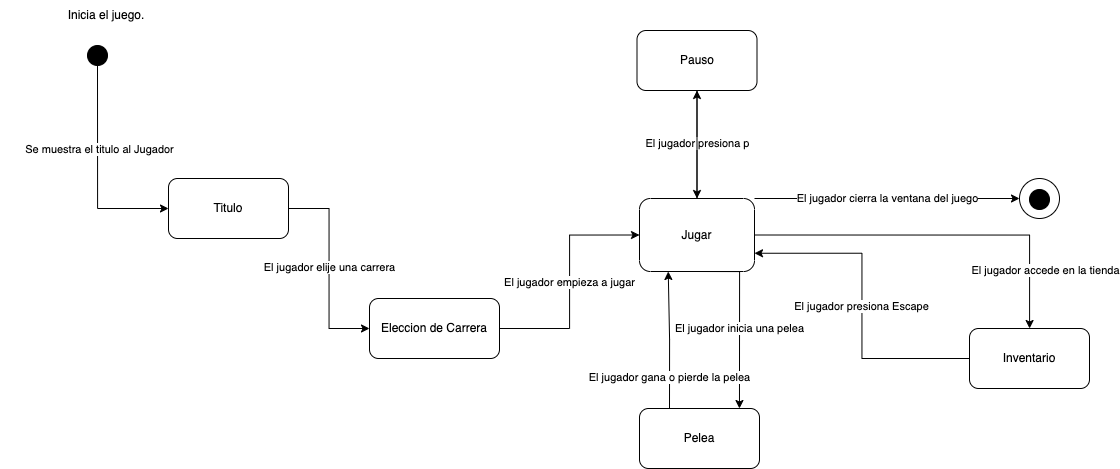
\includegraphics[scale=0.18]{./DiagramaEstadosInterfaz.png}
\end{center}

\subsection*{Diagrama de Secuencias:}
\begin{center}
  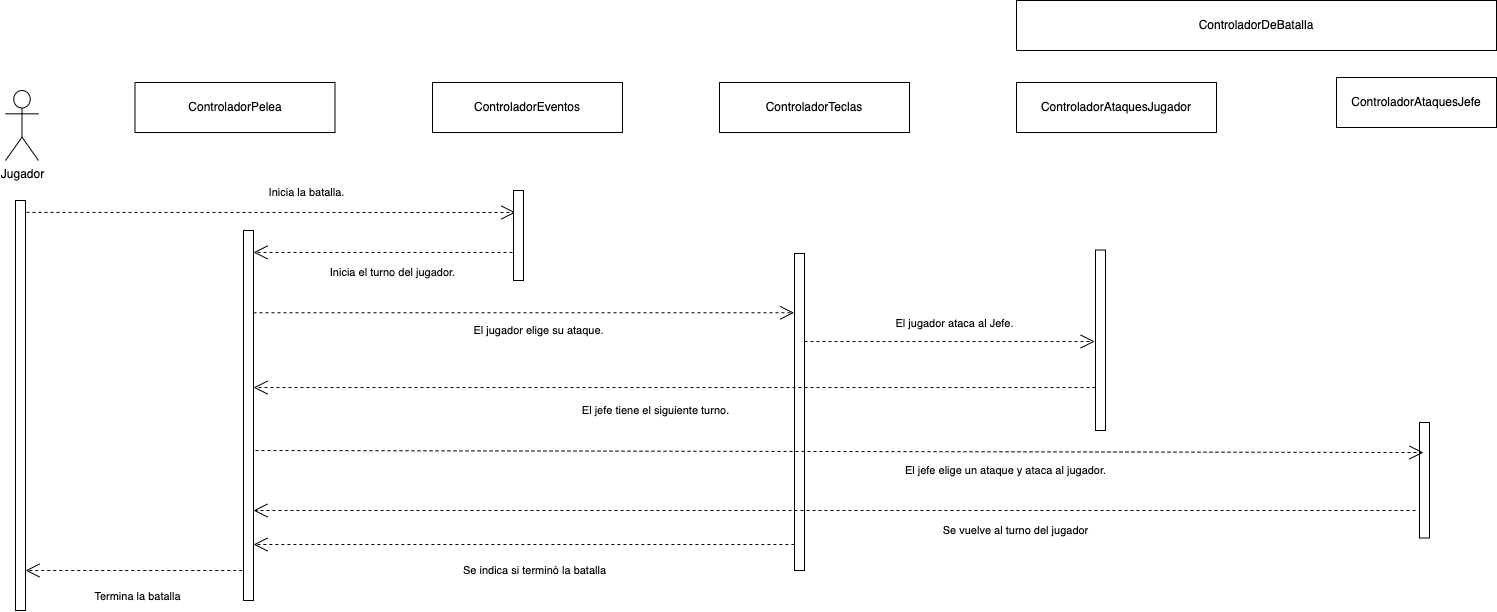
\includegraphics[scale=0.18]{./DiagramaDeSecuenciaDeBatalla.png}
\end{center}

\end{document}
